\section{大气压的测定}\label{sec:5-11}

大气压究竟有多大呢?在 17 世纪 40 年代,意大利科学家托里拆利用下面的实验首先测出了大气压的值。

\begin{figure}[htbp]
    \centering
    \begin{minipage}{9cm}
    \centering
    \vspace{5.5em}
    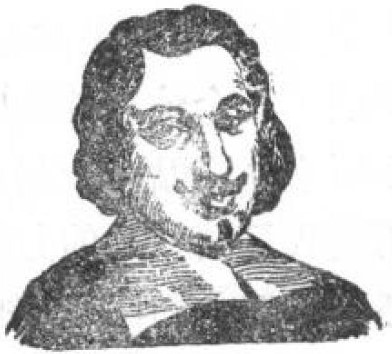
\includegraphics[width=6cm]{../pic/czwl1-ch5-torricelli}
    \caption*{托里拆利(1608 ~ 1647)}\label{fig:5-torricelli}
    \end{minipage}
    \qquad
    \begin{minipage}{5cm}
    \centering
    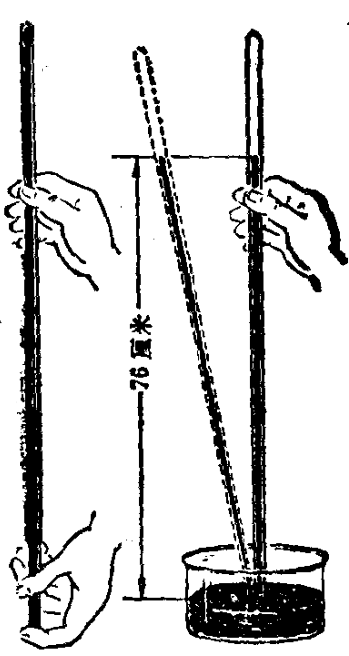
\includegraphics[width=4cm]{../pic/czwl1-ch5-41}
    \caption{托里拆利实验}\label{fig:5-41}
    \end{minipage}
\end{figure}


拿一根大约 1 米长的一端封闭的玻璃管,在管内灌满水银,然后用食指堵住开口的一端,把管倒立在水银槽里(图 \ref{fig:5-41})。
放开食指,管内的水银面就下降,降到管内的水银面比管外的水银面大约高 76 厘米时,就不再下降了。
如果使玻璃管倾斜,进到管里的水银就多一些,尽管这时水银柱的长度增加了,但是管内外水银面的高度差却保持不变,仍然是大约 76 厘米。

如果玻璃管的上端是开口的,管里水银面上就受到跟管外水银面上相同的大气压,依照连通器的道理,管内外的水银面就会相平。
现在管里水银面的上方没有空气,因此也就没有空气的压强作用在水银面上,而管外的水银面上却受到大气压的作用,
作用在管外水银面上的大气压就支持着管里的水银柱。可见,这个水银柱产生的压强就等于大气压。

因为管里的水银柱高大约是 76 厘米,所以大气压约等于 76 厘米高水银柱产生的压强。

根据液体压强的公式 $p = \rho gh$,水银的密度是 $13.6 \times 10^3 \qkmlfm$,
因此,76 厘米高水银柱产生的压强是
\begin{align*}
    p &= 13.6 \times 10^3 \qkmlfm \times 9.8 \ndmqk \times 0.76 \mi \\
      &= 1.01 \times 10^5 \ndmpfm = 1.01 \times 10^5 \pasika \;\juhao
\end{align*}

这就大约是大气压的值。这个压强大致相当于 1 千克的物体压在 $1 \pflm$ 面积上产生的压强,可见大气压是很大的。

因为水银柱的高度跟大气压的大小成正比,所以通常也直接用水银柱高度的毫米数来表示大气压的值。
如果水银高 760 毫米,我们就说大气压是 760 毫米汞柱\footnote{汞:读 \pinyin{gong3},是水银的化学名称。}。



\lianxi

(1) 用麦秆可以把瓶子中的水吸到嘴里(图 \ref{fig:5-42} 甲),这是为什么?
如果把玻璃管通过塞得很紧的橡皮塞插入盛水的瓶子里,用嘴吸玻璃管(图 \ref{fig:5-42} 乙),还能把水吸上来吗?

\begin{figure}[htbp]
    \centering
    \begin{minipage}{6cm}
    \centering
    \vspace{6em}
    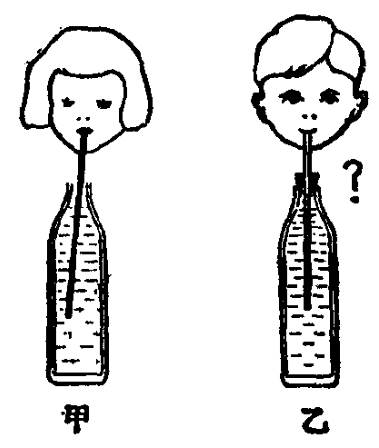
\includegraphics[width=5cm]{../pic/czwl1-ch5-42}
    \caption{}\label{fig:5-42}
    \end{minipage}
    \qquad
    \begin{minipage}{3cm}
    \centering
    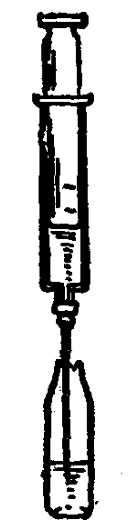
\includegraphics[width=2cm]{../pic/czwl1-ch5-43}
    \caption{}\label{fig:5-43}
    \end{minipage}
    \qquad
    \begin{minipage}{5cm}
    \centering
    \vspace{8em}
    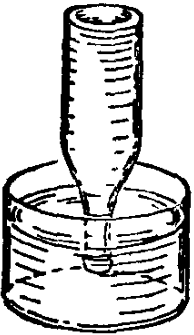
\includegraphics[width=3cm]{../pic/czwl1-ch5-44}
    \caption{}\label{fig:5-44}
    \end{minipage}
\end{figure}

(2) 自来水笔吸水时,把笔上的弹簧片按几下,墨水就吸到橡皮管里去了,这是什么原因?

(3) 医生打针时,先把针管里的活塞推到下端,然后把针头插入药液中,提起活塞,
药液就能进入针管里(图 \ref{fig:5-43})。解释这个现象。

(4) 在瓶子里灌满水,用塞子把瓶口塞住,然后把瓶子倒立在水中,拨掉瓶塞(图 \ref{fig:5-44}),
这时水会不会从瓶中流出来?做做看,并作出解释。

(5) 大气压也作用在每个人的身上,但是为什么没有把我们压瘪了?

(6) 房顶的面积是 $45\pfm$ ,大气作用在房顶上的压力是多大?这么大的力为什么没有把房顶压塌?

(7) 已知大气压的值,能不能利用公式 $p = \rho gh$,算出大气层的高度?为什么?


